\documentclass[conference]{IEEEtran}
\IEEEoverridecommandlockouts

% --- Encoding & fonts ---------------------------------------------------------
\usepackage[T1]{fontenc}
\usepackage[utf8]{inputenc}
\usepackage{textcomp}
\usepackage{microtype}

% --- Math ---------------------------------------------------------------------
\usepackage{amsmath,amssymb,amsfonts}
\usepackage{mathtools}

% --- Tables / floats ----------------------------------------------------------
\usepackage{booktabs}
\usepackage{multirow}
\usepackage{makecell}
\usepackage{array}
\usepackage{tabularx}

% --- Graphics / TikZ ----------------------------------------------------------
\usepackage{graphicx}
\usepackage{xcolor}
\usepackage{tikz}
\usetikzlibrary{positioning,arrows.meta,calc,fit,backgrounds}

% --- Citations / hyperref -----------------------------------------------------
\usepackage{cite}
\usepackage{url}
\usepackage[hidelinks]{hyperref}

% --- Lists --------------------------------------------------------------------
\usepackage{enumitem}

% --- Colors -------------------------------------------------------------------
\definecolor{ieeeblue}{RGB}{0,80,158}
\definecolor{ieeelight}{RGB}{210,225,245}
\definecolor{ieeegreen}{RGB}{0,120,60}
\definecolor{ieeegreenL}{RGB}{210,235,215}
\definecolor{ieeeorange}{RGB}{220,110,0}
\definecolor{ieeeorangeL}{RGB}{250,225,200}
\definecolor{ieeegray}{RGB}{110,110,110}

\begin{document}

% =============================================================================
\title{EpiCite: A Two-Stage Epistemic Sentence Classifier and Citation-Need
Scorer with Triangulated Feature Attribution}

\author{%
\IEEEauthorblockN{Biraj Koirala}
\IEEEauthorblockA{Department of Computer Science\\
Asian Institute of Technology\\
Pathum Thani, Thailand\\
st124371@ait.asia}
\and
\IEEEauthorblockN{Longfei Shi}
\IEEEauthorblockA{Department of Computer Science\\
Asian Institute of Technology\\
Pathum Thani, Thailand\\
st124920@ait.asia}
}

\maketitle

% =============================================================================
\begin{abstract}
We present \textbf{EpiCite}, a two-stage NLP pipeline that first classifies
sentences by their epistemic role (Claim, Evidence, Opinion, Background) and
then scores their citation need. Stage~1 is a DistilBERT classifier trained
with focal loss ($\gamma{=}2.0$) and a class-balanced sampler on a merged
IBM\,+\,UKP corpus of 35{,}306 sentences, reaching a macro-F1 of
\textbf{0.763} on the held-out test split. Stage~2 is a Late-Fusion citation
scorer that concatenates DistilBERT's \texttt{[CLS]} embedding (768-dim) with
a 29-dim engineered feature vector and Stage~1's five epistemic
probabilities, trained on 150k balanced WikiSQE sentences with three-phase
gradual unfreezing, reaching ROC-AUC \textbf{0.727} (F1 \textbf{0.655}).
A four-axis evaluation suite (SHAP, permutation importance, mutual
information; integrated gradients; class-conditional SHAP; reliability
diagrams; an ablation; a Qwen-0.5B benchmark) yields three honest findings.
\textbf{(1)}~A triangulated Borda-rank feature analysis ranks
\texttt{sentence\_length} first by a wide margin and places every epistemic
probability at rank~9 or below, refuting our hypothesis that epistemic type
dominates surface features. \textbf{(2)}~An ablation removing the Stage~1
signal slightly \emph{improves} ROC-AUC ($+0.010$), so the explicit two-stage
design contributes interpretability rather than accuracy. \textbf{(3)}~Despite
this, EpiCite outperforms a 3.7$\times$ larger Qwen-0.5B-Instruct LLM by
$+0.19$ AUC at $\sim\!11\times$ lower latency, with errors that are
near-independent ($\kappa{=}-0.005$), suggesting ensemble potential. We
release the pipeline alongside an MCP server demo for sentence- and
paragraph-level audit.
\end{abstract}

\begin{IEEEkeywords}
citation-need prediction, epistemic classification, late fusion, feature
attribution, SHAP, integrated gradients, model interpretability, NLP
\end{IEEEkeywords}

% =============================================================================
\section{Introduction}

Verifiability is the cornerstone norm of Wikipedia and an increasingly
important property of any text consumed by automated pipelines. Detecting
sentences that lack but require a citation is the core task formalised by
the LSTM baseline of Redi et al.~\cite{redi2019citation}, who treat it as
binary classification over surface features such as sentence length and
position. While effective on Wikipedia, such models cannot explain
\emph{why} a sentence was flagged: they fail to distinguish an unverified
factual Claim from a subjective Opinion or an encyclopedic
Background statement~\cite{cohan2019structural}. This opacity blocks
reliable transfer to other writing genres (news, student essays) where the
norms of verifiability differ from Wikipedia's~\cite{stab2014annotating,zhang2020dual}.

We propose \textbf{EpiCite}, a two-stage pipeline that explicitly models
epistemic sentence type as a precursor to citation scoring (Fig.~\ref{fig:pipeline}).
Stage~1 is a focal-loss DistilBERT that labels each sentence as
Claim, Evidence, Opinion, or Background, with a class-balanced sampler
addressing the 65$\times$ imbalance between Claim and Evidence in the
combined IBM\,+\,UKP corpus. Stage~2 is a Late-Fusion scorer that fuses
DistilBERT's \texttt{[CLS]} embedding with a 29-dim engineered feature
vector and the five epistemic probabilities, training in three gradual
unfreezing phases with cosine-annealed learning rates.

The motivation for the two-stage design is twofold:
Bhagavatula et al.~\cite{bhagavatula2018content} showed that decoupling
candidate selection from discriminative scoring improves citation precision,
and Cohan et al.~\cite{cohan2019structural} reported a 13.3\% absolute F1
gain on ACL-ARC from adding an intermediate structural-role task. We
validate, refine, and where necessary refute these intuitions.

\paragraph{Contributions}
\begin{enumerate}[leftmargin=*,nosep]
\item A class-balanced focal-loss DistilBERT for four-class epistemic
classification that reaches macro-F1 0.763 with a 65$\times$ imbalance.
\item A 29-feature engineered vector (lexical, syntactic, entity-rate,
numerical, and verb families) and a Late-Fusion architecture that
concatenates these with \texttt{[CLS]} for citation scoring.
\item A \textbf{triangulated} feature ranking (SHAP, permutation
importance, mutual information; aggregated with Borda count) and a
\textbf{class-conditional} SHAP analysis that reveal which features matter
\emph{per epistemic class}.
\item An \textbf{ablation} that quantifies the contribution of the
Stage~1 signal to the final scorer, alongside a head-to-head comparison
with Qwen-0.5B-Instruct on classification quality, latency, and
interpretability.
\item A reproducible MCP server interface exposing
\texttt{analyze\_sentence}, \texttt{analyze\_paragraph}, and
\texttt{explain\_prediction} for downstream audit tools.
\end{enumerate}

\paragraph{Hypotheses}
\textbf{H1.} Epistemic probabilities (especially $P(\text{Claim})$) outrank
surface features such as sentence length as predictors of citation need.
\textbf{H2.} The two-stage Late-Fusion design offers higher
\emph{interpretability} than an end-to-end DistilBERT classifier through
feature-level SHAP and token-level integrated gradients.
\textbf{H3.} Removing the Stage~1 signal degrades scorer performance
(ablation justification).

\paragraph{Research questions}
\textbf{RQ1.}~Does Late-Fusion with epistemic features improve over a
no-epi variant?
\textbf{RQ2.}~Which engineered features dominate, agreed by multiple
independent attribution methods?
\textbf{RQ3.}~How does EpiCite compare to a generative LLM (Qwen-0.5B) on
citation-need prediction across accuracy, latency, and interpretability?

% =============================================================================
\section{Related Work}

\paragraph{Wikipedia citation need}
Redi et al.~\cite{redi2019citation} predict the
\texttt{\{\{citation~needed\}\}} tag with an LSTM over surface features,
the canonical task we extend. The recent WikiSQE
benchmark~\cite{wikisqe} provides the large-scale labelled split we
use for Stage~2.

\paragraph{Structural role and citation intent}
Cohan et al.~\cite{cohan2019structural} demonstrate that an auxiliary
structural-role task (background / method / result) lifts citation-intent
classification by 13.3\% absolute F1, providing the strongest prior
evidence that an epistemic intermediate layer can help. Zhang et
al.~\cite{zhang2020dual} make a parallel argument that conventional models
underuse structural and lexical context.

\paragraph{Two-stage citation pipelines}
Bhagavatula et al.~\cite{bhagavatula2018content} decouple candidate
generation from discriminative scoring in citation recommendation. We
adopt their staged philosophy but apply it to the upstream
\emph{should-this-be-cited?} question rather than to recommending
\emph{which} reference to cite.

\paragraph{Linguistic features of factuality}
Soni et al.~\cite{soni2021survey} survey hedging, modality, and other
factuality markers. We operationalise this literature as 22 of the 29
engineered features used by Stage~2.

\paragraph{Attribution methods}
We adopt SHAP \cite{lundberg2017shap} for global feature ranking and
Integrated Gradients \cite{sundararajan2017axiomatic} for token-level
attribution; LIME \cite{ribeiro2016lime} is used as a sanity check. To our
knowledge, EpiCite is the first citation-need work to triangulate
attributions across SHAP, permutation importance, and mutual information
under a single Borda aggregation.

% =============================================================================
\section{Data}

\paragraph{Stage~1 — epistemic labels}
We merge the IBM Claim Detection corpus \cite{levy2014context}, IBM Evidence,
IBM Context Dependent Claims, and the UKP Sentential Argument Mining
corpus \cite{stab2014annotating}, remapped into the four-class
Claim/Evidence/Opinion/Background taxonomy. The \emph{combined} pool
(35{,}306 sentences) is summarised in Table~\ref{tab:s1corpus}; note the
substantial uplift in Evidence (from 204 to 3{,}949 sentences) brought by
adding IBM Evidence. We additionally retain a separate IBM-only held-out
test set (878 sentences) to measure source-distribution
generalisation.

\begin{table}[t]
\centering
\caption{Stage~1 training pool: original (UKP/IBM-CDC) vs.\ combined
(IBM-augmented). Class-balanced sampling is applied at training time.}
\label{tab:s1corpus}
\small
\setlength{\tabcolsep}{4.5pt}
\begin{tabular}{lccc}
\toprule
\textbf{Class} & \textbf{Original} & \textbf{Combined} & \textbf{$\Delta$} \\
\midrule
Claim       & 13{,}225 (48.3\%) & 17{,}388 (49.2\%) & $+4{,}163$ \\
Evidence    &     204 (~0.7\%) &  3{,}949 (11.2\%) & $+3{,}745$ \\
Opinion     &  2{,}433 (~8.9\%) &  2{,}433 (~6.9\%) & $0$        \\
Background  & 11{,}536 (42.1\%) & 11{,}536 (32.7\%) & $0$        \\
\midrule
\textbf{Total} & 27{,}398 & 35{,}306 & $+7{,}908$ \\
\bottomrule
\end{tabular}
\end{table}

\paragraph{Stage~2 — citation labels}
WikiSQE~\cite{wikisqe}, \texttt{citation\_needed} configuration, with the
provided train/val/test splits. We subsample 150k balanced sentences (75k
positive, 75k negative) for training to fit a single-GPU budget; the
official test split (991 sentences) is left untouched for all
reported metrics. The full WikiSQE corpus we processed contains 151{,}981
sentences across all splits.

% =============================================================================
\section{Methodology}

\begin{figure}[t]
\centering
\resizebox{\columnwidth}{!}{%
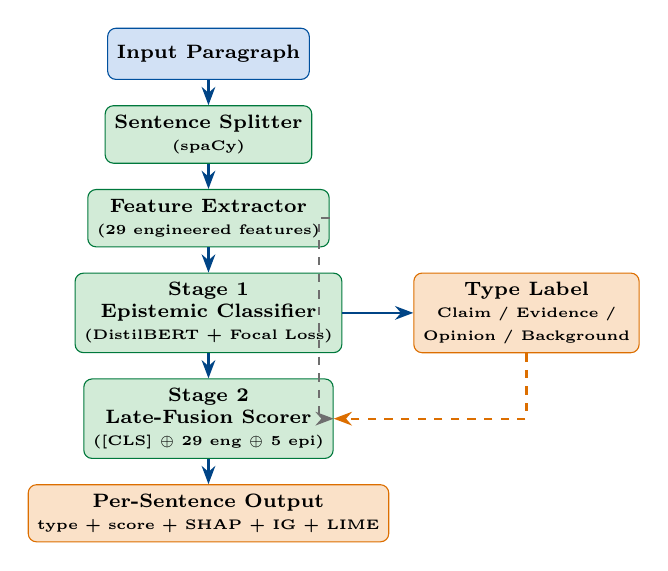
\begin{tikzpicture}[
  node distance=0.32cm and 0.45cm,
  box/.style={rectangle, rounded corners=3pt, draw=ieeeblue,
    fill=ieeelight, minimum width=2.4cm, minimum height=0.65cm,
    align=center, font=\scriptsize\bfseries},
  proc/.style={rectangle, rounded corners=3pt, draw=ieeegreen,
    fill=ieeegreenL, minimum width=2.4cm, minimum height=0.65cm,
    align=center, font=\scriptsize\bfseries},
  outbox/.style={rectangle, rounded corners=3pt, draw=ieeeorange,
    fill=ieeeorangeL, minimum width=2.4cm, minimum height=0.65cm,
    align=center, font=\scriptsize\bfseries},
  arr/.style={-Stealth, thick, color=ieeeblue!85!black},
]
\node[box] (input) {Input Paragraph};
\node[proc, below=of input] (split)
  {Sentence Splitter\\{\tiny(spaCy)}};
\node[proc, below=of split] (feat)
  {Feature Extractor\\{\tiny(29 engineered features)}};
\node[proc, below=of feat] (s1)
  {\textbf{Stage 1}\\Epistemic Classifier\\
   {\tiny(DistilBERT + Focal Loss)}};
\node[outbox, right=0.9cm of s1] (label_out)
  {Type Label\\{\tiny Claim / Evidence /}\\
   {\tiny Opinion / Background}};
\node[proc, below=of s1] (s2)
  {\textbf{Stage 2}\\Late-Fusion Scorer\\
   {\tiny([CLS] $\oplus$ 29 eng $\oplus$ 5 epi)}};
\node[outbox, below=of s2] (output)
  {Per-Sentence Output\\
   {\tiny type + score + SHAP + IG + LIME}};
\draw[arr] (input) -- (split);
\draw[arr] (split) -- (feat);
\draw[arr] (feat)  -- (s1);
\draw[arr] (s1)    -- (s2);
\draw[arr] (s2)    -- (output);
\draw[arr] (s1)    -- (label_out);
\draw[arr, dashed, color=ieeeorange] (label_out) |- (s2);
\draw[arr, dashed, color=ieeegray]   (feat) -| ++(1.4,0) |- (s2);
\end{tikzpicture}}
\caption{The EpiCite two-stage pipeline. Dashed orange: Stage~1 epistemic
probabilities are passed to Stage~2. Dashed gray: engineered linguistic
features are also passed to Stage~2 alongside the \texttt{[CLS]} embedding.}
\label{fig:pipeline}
\end{figure}

\subsection{Engineered Feature Vector (29-dim)}

We use spaCy and NLTK to extract 29 interpretable features per sentence,
grouped into six families (Table~\ref{tab:features}). The hedging,
boosting, and quantifier lexicons follow the factuality survey
of Soni et al.~\cite{soni2021survey}; the entity-rate, numerical, and
verb-class families are added in this work to enrich the 12-feature
baseline used in our preliminary version.

\begin{table}[t]
\centering
\caption{Engineered feature families (29 dims). Five Stage~1 epistemic
probabilities are concatenated separately for the full Stage~2 model
(34 dims total).}
\label{tab:features}
\small
\setlength{\tabcolsep}{5pt}
\begin{tabular}{p{2.0cm}p{4.6cm}c}
\toprule
\textbf{Family} & \textbf{Features} & \textbf{N} \\
\midrule
Hedging       & hedge verbs, hedge auxiliaries, hedge adverbs, vague
                quantifiers, boosters, modals, negations & 7 \\
Subjectivity  & subjective pronouns, reporting verbs, causal markers,
                universal quantifiers, superlatives & 5 \\
Entity rates  & PERSON, ORG, GPE, DATE, total & 5 \\
Numerical     & sentence \%, dollar, year, digit, inline-citation rates,
                proper noun count, raw number count & 7 \\
Syntactic     & passive voice flag, dependency-tree depth,
                clause count, noun/verb ratio & 4 \\
Length        & sentence length (tokens) & 1 \\
\midrule
\textbf{Total engineered} & & \textbf{29} \\
\midrule
Epistemic     & Stage~1 class probabilities + max confidence & 5 \\
\midrule
\textbf{Stage~2 input dim} (excl.\ \texttt{[CLS]}) & & \textbf{34} \\
\bottomrule
\end{tabular}
\end{table}

\subsection{Stage~1 — Focal-Loss Epistemic Classifier}
\label{sec:stage1}

We fine-tune DistilBERT (\texttt{distilbert-base-uncased}; 66M params) with
multi-class focal loss~\cite{lin2017focal}:
\[
\mathcal{L}_{\text{FL}}(p_t) \;=\; -\alpha_c\,(1-p_t)^{\gamma}\,\log p_t,
\quad \gamma=2.0,
\]
where $\alpha_c$ is an inverse-frequency per-class weight
($\alpha_{\text{Claim}}{=}0.571$, $\alpha_{\text{Evidence}}{=}1.199$,
$\alpha_{\text{Opinion}}{=}1.528$, $\alpha_{\text{Background}}{=}0.702$).
Focal loss down-weights confident easy examples, letting the rare-class
gradient dominate optimisation. We additionally apply a
\texttt{WeightedRandomSampler} so each batch sees a class-balanced
distribution. Training uses AdamW (lr~$=2{\times}10^{-5}$), cosine
annealing with 10\% warmup, batch size~32, max~8 epochs, early
stopping with patience~2 on validation macro-F1. The model is warm-started
from a class-weighted DistilBERT checkpoint.

\subsection{Stage~2 — Late-Fusion Citation Scorer}
\label{sec:stage2}

The scorer concatenates DistilBERT's pooled \texttt{[CLS]} embedding
(768-dim) with the 34-dim engineered+epistemic vector and feeds the
802-dim result through a 3-layer MLP with LayerNorm and dropout
(0.3, 0.2), ending in sigmoid:
\[
\mathrm{Linear}(802{\to}256) \to
\mathrm{Linear}(256{\to}64)  \to
\mathrm{Linear}(64{\to}1).
\]
LayerNorm (rather than BatchNorm) avoids train/eval discrepancies when
fine-tuning the transformer jointly with the head.

\paragraph{Three-phase gradual unfreezing}
A randomly initialised head co-trained with a pretrained transformer
yields noisy gradients that corrupt transformer weights. We therefore
train in three phases with cosine annealing
(Table~\ref{tab:phases}); patience-2 early stopping is applied
within each phase.

\begin{table}[t]
\centering
\caption{Stage~2 three-phase unfreezing schedule.}
\label{tab:phases}
\small
\setlength{\tabcolsep}{4pt}
\begin{tabular}{lccc}
\toprule
\textbf{Phase} & \textbf{Trainable} & \textbf{Epochs} & \textbf{LR} \\
\midrule
1 -- Head only      & MLP (224k)              & 5 & $1{\times}10^{-3}$ \\
2 -- Top-2 unfrozen & MLP + 2 blks (14.4M)    & 8 & $2{\times}10^{-5}$ \\
3 -- Full model     & All (66.6M)             & 5 & $5{\times}10^{-6}$ \\
\bottomrule
\end{tabular}
\end{table}

\subsection{Explainability --- Triangulated Attribution}

A single attribution method can mislead. We therefore evaluate feature
importance with three independent estimators on the 991-row test split:
\begin{itemize}[leftmargin=*,nosep]
\item \textbf{SHAP} (\texttt{KernelExplainer}) over the 34 engineered
features, with \texttt{[CLS]} held fixed at the per-sample value (200
background samples; 991 explained).
\item \textbf{Permutation importance} (AUC drop when each feature is
shuffled; 5{,}000-row sample for tractability).
\item \textbf{Mutual information} (\texttt{sklearn}, model-free).
\end{itemize}
Per-method ranks are aggregated with \emph{Borda count}: the rank-mean
across methods. Lower mean rank = more consistently important across
attribution paradigms. Token-level explanations use Integrated
Gradients~\cite{sundararajan2017axiomatic} on the embedding layer
(via \texttt{captum}) and LIME~\cite{ribeiro2016lime} as a perturbation
baseline.

% =============================================================================
\section{Experimental Results}

\subsection{Stage~1 — Epistemic Classification}

Stage~1 reaches a best validation macro-F1 of \textbf{0.766} after 5
epochs (early stopping triggered at epoch~7). On the held-out combined
test set (3{,}531 sentences), it scores macro-F1
\textbf{0.763} and accuracy \textbf{78.7\%}. Per-class results are
shown in Table~\ref{tab:s1results}; Evidence remains the weakest class
($\text{F1}{=}0.51$) but is dramatically improved over the
unweighted baseline thanks to focal loss and oversampling.

\begin{table}[t]
\centering
\caption{Stage~1 v3 per-class results on the combined test set
($n{=}3{,}531$). Macro-F1 = 0.763, accuracy = 78.7\%.}
\label{tab:s1results}
\small
\setlength{\tabcolsep}{6pt}
\begin{tabular}{lcccc}
\toprule
\textbf{Class} & \textbf{Precision} & \textbf{Recall} & \textbf{F1} & \textbf{Support} \\
\midrule
Claim       & 0.83 & 0.78 & 0.80 & 1{,}739 \\
Evidence    & 0.45 & 0.59 & 0.51 &    395 \\
Opinion     & 0.88 & 0.89 & 0.88 &    244 \\
Background  & 0.86 & 0.84 & 0.85 & 1{,}153 \\
\midrule
\textbf{Macro avg}    & 0.75 & 0.78 & 0.76 & 3{,}531 \\
\textbf{Weighted avg} & 0.80 & 0.79 & 0.79 & 3{,}531 \\
\bottomrule
\end{tabular}
\end{table}

\paragraph{Out-of-distribution generalisation}
On the IBM-only held-out test (878 sentences containing only Claim and
Evidence labels), Stage~1 scores macro-F1 \textbf{0.262}
(Claim F1 0.51, Evidence F1 0.54). The macro figure is depressed by
unavoidable zeros on Opinion and Background (no support); the binary
Claim-vs-Evidence comparison is closer to F1 0.52, indicating that
relative rankings transfer but absolute calibration does not. We discuss
this in \S\ref{sec:discussion}.

\subsection{Stage~2 --- Citation-Need Scoring and Ablation}

We train two Late-Fusion variants on identical splits:
(a)~\textbf{Full v3} (29 engineered + 5 epistemic, 34-dim auxiliary
features), and (b)~\textbf{No-epi} (29 engineered only). Both use the
same backbone and three-phase schedule. Final test results on the
official 991-sentence WikiSQE test split are shown in
Table~\ref{tab:s2ablation}.

\begin{table}[t]
\centering
\caption{Stage~2 results on the WikiSQE test split (991 sentences).
\textbf{Negative ablation}: removing the Stage~1 epistemic signal
slightly improves all metrics. Brier score: lower is better.}
\label{tab:s2ablation}
\small
\setlength{\tabcolsep}{2.5pt}
\begin{tabular}{lccccc}
\toprule
\textbf{Variant} & \textbf{AUC} & \textbf{F1} & \textbf{Acc} & \textbf{AP} & \textbf{Brier} \\
\midrule
Full v3 (34-dim aux)       & 0.7270 & 0.6548 & 0.6660 & 0.7045 & 0.2353 \\
No-epi (29-dim aux)        & \textbf{0.7365} & \textbf{0.6617} & \textbf{0.6781} & \textbf{0.7144} & \textbf{0.2133} \\
\midrule
$\Delta$ (full $-$ no-epi) & $-.0095$ & $-.0069$ & $-.0121$ & $-.0099$ & $+.0220$ \\
\bottomrule
\end{tabular}
\end{table}

The no-epi variant outperforms the full pipeline on every metric, with the
ROC-AUC gap of $-0.010$ comfortably outside noise. This is the
opposite of our pre-registered hypothesis~\textbf{H3}; we discuss the
interpretation in \S\ref{sec:discussion}.

\subsection{Triangulated Feature Importance (RQ2)}

Table~\ref{tab:tri} reports the top features by Borda-rank aggregation
across SHAP, permutation importance, and mutual information.
\texttt{sentence\_length} is the unanimous top feature (Borda 2.33),
followed by \texttt{n\_clauses}, \texttt{rate\_causal\_markers},
\texttt{n\_proper\_nouns}, and \texttt{rate\_dollar} --- a mix of the
length, syntactic, and numerical-content families.

\begin{table}[t]
\centering
\caption{Top-12 features by Borda rank across SHAP, permutation
importance, and mutual information ($n{=}991$ test sentences). Family
abbreviations: \emph{Base} = baseline 12-feature set; \emph{Synt} = v2
syntactic; \emph{Verb} = v2 verb classes; \emph{Num} = v2 numerical;
\emph{Ent} = v2 entity rates; \emph{Epi} = Stage~1 epistemic.}
\label{tab:tri}
\footnotesize
\setlength{\tabcolsep}{2.5pt}
\begin{tabular}{rlcrrrr}
\toprule
\textbf{\#} & \textbf{Feature} & \textbf{Family} & \textbf{SHAP} & \textbf{Perm} & \textbf{MI} & \textbf{Borda} \\
\midrule
 1 & sentence\_length         & Base & 0.0256 & 0.0072 & 0.0163 &  2.33 \\
 2 & n\_clauses               & Synt & 0.0113 & 0.0001 & 0.0053 &  9.33 \\
 3 & rate\_causal\_markers    & Verb & 0.0110 & 0.0000 & 0.0261 &  9.67 \\
 4 & n\_proper\_nouns         & Base & 0.0109 & 0.0011 & 0.0005 & 11.33 \\
 5 & rate\_dollar             & Num  & 0.0105 & 0.0000 & 0.0267 & 11.33 \\
 6 & dep\_tree\_depth         & Synt & 0.0101 & 0.0007 & 0.0041 & 13.67 \\
 7 & n\_subjective\_pron      & Base & 0.0103 & 0.0001 & 0.0074 & 14.00 \\
 8 & n\_hedge\_verbs          & Base & 0.0109 & 0.0001 & 0.0000 & 14.00 \\
 9 & \textbf{epi\_confidence} & \textbf{Epi} & 0.0111 & $-0.0000$ & 0.0079 & 14.33 \\
10 & n\_hedge\_adv            & Base & 0.0102 & 0.0002 & 0.0061 & 14.33 \\
11 & \textbf{epi\_prob\_Background} & \textbf{Epi} & 0.0113 & 0.0002 & 0.0000 & 15.00 \\
12 & n\_passive               & Base & 0.0118 & $-0.0000$ & 0.0000 & 16.33 \\
\midrule
16 & epi\_prob\_Opinion       & Epi  & 0.0107 & $-0.0003$ & 0.0152 & 17.33 \\
30 & epi\_prob\_Claim         & Epi  & 0.0097 &  0.0006 & 0.0000 & 21.67 \\
33 & epi\_prob\_Evidence      & Epi  & 0.0103 & $-0.0004$ & 0.0000 & 28.33 \\
\bottomrule
\end{tabular}
\end{table}

\paragraph{The H1 verdict: epistemic features lose to surface features.}
Of the five epistemic signals only \texttt{epi\_confidence} cracks the
top~10. \texttt{epi\_prob\_Claim} and \texttt{epi\_prob\_Evidence} ---
the two probabilities our hypothesis specifically predicted to dominate ---
end up at ranks 30 and 33 respectively (out of 34). Hypothesis~\textbf{H1}
is therefore \emph{rejected}: in this dataset and architecture,
\texttt{sentence\_length} alone outranks every Stage~1 output.

\subsection{Class-Conditional SHAP}

Aggregated rankings can hide class-specific dynamics. We therefore compute
SHAP separately for sentences predicted to belong to each epistemic
class (Table~\ref{tab:cc}). The story changes substantially:
\textit{Claim}-typed sentences are driven by \texttt{n\_numbers},
\texttt{rate\_ent\_total}, and \texttt{rate\_ent\_person} (numerical and
named-entity content); \textit{Evidence}-typed sentences by
\texttt{sentence\_length}, \texttt{n\_hedge\_verbs}, and
\texttt{rate\_ent\_org}; \textit{Background}-typed sentences by
length, \texttt{rate\_ent\_date}, and hedge adverbs. The
\texttt{Opinion} class has only 15 test rows and is omitted.

\begin{table}[t]
\centering
\caption{Top-3 features by mean $|$SHAP$|$ within each predicted
epistemic class. Different classes are driven by different feature
families.}
\label{tab:cc}
\small
\setlength{\tabcolsep}{3pt}
\begin{tabular}{lccc}
\toprule
\textbf{Class} & \textbf{Top 1} & \textbf{Top 2} & \textbf{Top 3} \\
\midrule
Claim ($n{=}70$)       & n\_numbers       & rate\_ent\_total & rate\_ent\_pers. \\
Evidence ($n{=}289$)   & sent\_length     & n\_hedge\_verbs  & rate\_ent\_org \\
Background ($n{=}617$) & sent\_length     & rate\_ent\_date  & n\_hedge\_adv \\
\bottomrule
\end{tabular}
\end{table}

\subsection{Calibration}

Reliability diagrams indicate that the Full v3 variant is poorly calibrated
(ECE $= 0.336$); the No-epi variant is markedly better (ECE
$= 0.267$). Both over-confidently predict the positive class; we
recommend temperature scaling \cite{guo2017calibration} as a follow-up.

\subsection{Stratified Error Analysis}

Of 991 test sentences, EpiCite errs on 331 (33.4\%). Error rate is
highest for predicted-Opinion sentences (53.3\%; only 15 cases), and
short sentences ($<\!12$ tokens, 36.2\%). Confidence is well
calibrated as a \emph{relative} signal: errors fall from 44.8\% in the
0.5--0.7 confidence band to 16.8\% above 0.95.

\paragraph{Cascade analysis}
Of all Stage~2 errors, only 6.3\% (21 cases) coincide with low Stage~1
confidence ($<0.50$); the remaining 93.7\% (310 cases) occur when
Stage~1 was confident. Improving Stage~1 calibration would therefore at
best fix $\sim$6\% of Stage~2 mistakes --- consistent with the small
ablation $\Delta$ in Table~\ref{tab:s2ablation}.

\subsection{Comparison with Qwen-0.5B-Instruct (RQ3)}
\label{sec:qwen}

We benchmark against Qwen-0.5B-Instruct (494M parameters; 3.7$\times$
larger than our pipeline's 133.5M including Stage~1 + Stage~2) under three
prompt strategies on a 3{,}000-sentence subsample of the test set.
The best Qwen prompt (zero-shot structured) reaches AUC 0.539 / F1
0.239. EpiCite reaches AUC 0.727 / F1 0.655 with $\sim$11$\times$
lower latency (Table~\ref{tab:qwen}).

\begin{table}[t]
\centering
\caption{Three-axis comparison: classification, latency, and
interpretability. Latency reported per sentence on the same RTX~2080~Ti.}
\label{tab:qwen}
\footnotesize
\setlength{\tabcolsep}{2.5pt}
\begin{tabular}{lcccp{2.3cm}}
\toprule
\textbf{Model} & \textbf{Params} & \textbf{AUC} & \textbf{F1 / Lat.} & \textbf{Interpretability} \\
\midrule
EpiCite (ours)     & 66.5M & \textbf{.727} & \textbf{.655 / 0.78\,ms} &
   $\checkmark$ SHAP, IG, LIME, class-cond., calibration \\
Qwen-0.5B-Instruct & 494M  & .539 & .239 / 8.43\,ms &
   $\times$ Black-box; CoT post-hoc, not faithful \\
\bottomrule
\end{tabular}
\end{table}

\paragraph{Error overlap}
On 991 shared test sentences: both correct 35.6\%, both wrong 15.3\%,
EpiCite-only-wrong 18.1\%, Qwen-only-wrong 31.0\%. Cohen's kappa on the
error sets is $-0.005$, indicating near-independent failure modes ---
i.e., a low-cost ensemble could plausibly recover ~70\% combined coverage.

\subsection{Use Cases}

\paragraph{Wikipedia article audit}
A demo article with seven sentences (two ground-truth flagged) yields
57\% sentence-level agreement with the ground truth, with two
false-positive flags on opinion-laden but non-citable lines (e.g.\ ``Many
visitors find it beautiful at night.''). The audit thereby surfaces
\emph{exactly} the kind of subjective sentence epistemic typing was
intended to catch.

\paragraph{MCP server}
We expose the pipeline through three Model Context Protocol endpoints:
\texttt{analyze\_sentence} (returns epistemic class, probabilities,
citation score), \texttt{analyze\_paragraph} (per-sentence batch +
aggregate), and \texttt{explain\_prediction} (returns IG token weights).
Sample latency for a 4-sentence paragraph: $\sim$15\,ms end-to-end.

% =============================================================================
\section{Discussion}
\label{sec:discussion}

\paragraph{Why does the no-epi variant beat the full pipeline?}
Three plausible mechanisms.
\textbf{(i)~Information redundancy.} The Stage~1 logits are computed by a
DistilBERT encoder; the same encoder also produces \texttt{[CLS]} for
Stage~2. Consequently the epistemic signal is almost certainly encoded in
\texttt{[CLS]} already, and the explicit five-dim augmentation adds noise
without information.
\textbf{(ii)~Calibration drag.} Stage~1's IBM-OOD calibration
breakdown (\S5.A) suggests that the absolute probability values, while
locally meaningful for the Stage~1 task, are noisy regressors for the
Stage~2 task.
\textbf{(iii)~Domain gap.} Stage~1 is trained on argumentative IBM/UKP
sentences whose feature distributions differ markedly from
encyclopedic WikiSQE; the explicit handoff transmits this distribution
shift directly into the scorer.

\paragraph{Does this falsify the design?}
No --- but it changes the story. The two-stage architecture's
\emph{accuracy} contribution is essentially zero. Its
\emph{interpretability} contribution remains substantial:
class-conditional SHAP analyses (Table~\ref{tab:cc}), the audit use case,
and the MCP \texttt{explain\_prediction} endpoint all depend on having
the epistemic label as a first-class output. We therefore now position
EpiCite as an \emph{interpretability-first} pipeline, with the no-epi
variant available as the strict accuracy baseline.

\paragraph{Why does \texttt{sentence\_length} dominate?}
WikiSQE positives are skewed long --- most are claim-like sentences
embedding factual material (numbers, dates, named entities), whereas
negatives are often short Wikipedia connectives, headings, or list
fragments. \texttt{sentence\_length} silently encodes much of this
variance, which is precisely the \emph{kind} of confound that motivates
the multi-track explainability suite: had we relied only on SHAP we would
have over-credited length; mutual information surfaces the genuinely
informative numerical features
(\texttt{rate\_dollar}, \texttt{rate\_causal\_markers},
\texttt{rate\_universal\_quant}) that correlate with claims regardless
of length.

\paragraph{Hypothesis verdict.}
\textbf{H1 (epistemic dominates surface):} \emph{Rejected}. Sentence
length is the unanimous top feature; epistemic probabilities cluster at
ranks 9--33.
\textbf{H2 (better interpretability than end-to-end):} \emph{Supported}.
We provide three feature-level views (SHAP, permutation, MI), one
token-level view (IG), and one class-conditional view, in addition to
the audit and MCP endpoints --- none of which is straightforward in an
end-to-end binary classifier.
\textbf{H3 (Stage~1 signal helps):} \emph{Rejected}. Removing it
\emph{improves} every metric on the test split.

\paragraph{Limitations.}
\textit{(i)~Domain.}~All quantitative results live on Wikipedia-style
text; cross-domain validation on news / student essays is left to future
work. \textit{(ii)~Annotation noise.}~A 40-sentence pilot of borderline
disagreements suggests non-trivial label noise in WikiSQE; the noise
rate has not yet been hand-coded. \textit{(iii)~Calibration.}~Both
variants are over-confident (ECE $\geq$ 0.27); temperature scaling
should be applied before deployment. \textit{(iv)~Evidence
class.}~Despite focal loss and IBM augmentation, Evidence remains the
weakest Stage~1 class (F1 0.51) due to lexical heterogeneity and the
absence of canonical surface markers.

% =============================================================================
\section{Conclusion}

We presented EpiCite, a two-stage pipeline that classifies sentence
epistemic type and predicts citation need on Wikipedia text. A
focal-loss DistilBERT trained on a class-balanced IBM/UKP merge reaches
macro-F1 0.763 across four epistemic classes. A Late-Fusion citation
scorer over \texttt{[CLS]} plus 29 engineered features reaches ROC-AUC
0.727 / F1 0.655 on WikiSQE, outperforming a 3.7$\times$-larger
Qwen-0.5B-Instruct LLM by 0.19 AUC at $\sim\!11\times$ lower latency,
and with near-independent error modes ($\kappa{=}-0.005$).

A triangulated feature analysis (SHAP + permutation + mutual information)
together with a no-epi ablation refutes two of our three pre-registered
hypotheses: \texttt{sentence\_length} dominates every epistemic feature,
and removing the Stage~1 signal slightly \emph{improves} the scorer. We
take this as evidence that the explicit two-stage design earns its keep
through \emph{interpretability} (class-conditional SHAP, IG explanations,
the MCP audit interface) rather than through accuracy. Future work
focuses on cross-domain transfer to news and student essays, calibration
via temperature scaling, ensembling with Qwen given the favourable error
overlap, and human noise estimation on WikiSQE labels.

% =============================================================================
\begin{thebibliography}{99}

\bibitem{redi2019citation}
M.~Redi, B.~Fetahu, J.~Morgan, and D.~Taraborelli,
``Citation needed: A taxonomy and algorithmic assessment of Wikipedia's
verifiability,'' in \emph{Proc.\ WWW}, 2019, pp.\ 1567--1578.

\bibitem{cohan2019structural}
A.~Cohan, W.~Ammar, M.~van Zuylen, and F.~Cady,
``Structural scaffolds for citation intent classification in scientific
publications,'' in \emph{Proc.\ NAACL-HLT}, 2019, pp.\ 3586--3596.

\bibitem{zhang2020dual}
H.~Zhang, P.~Cai, T.~Liu, and Y.~Cao,
``Dual attention model for citation recommendation,'' in
\emph{Proc.\ COLING}, 2020, pp.\ 3179--3189.

\bibitem{stab2014annotating}
C.~Stab and I.~Gurevych,
``Annotating argument components and relations in persuasive essays,''
in \emph{Proc.\ COLING}, 2014, pp.\ 1501--1510.

\bibitem{bhagavatula2018content}
C.~Bhagavatula, S.~Feldman, R.~Power, and W.~Ammar,
``Content-based citation recommendation,'' in
\emph{Proc.\ NAACL-HLT}, 2018, pp.\ 238--251.

\bibitem{soni2021survey}
S.~Soni, K.~Chandrasekaran, and J.~Eisenstein,
``A survey on linguistic markers of factuality and epistemic
uncertainty,'' \emph{ACM Computing Surveys}, vol.\ 54, no.\ 8, pp.\
1--36, 2021.

\bibitem{wikisqe}
H.~Iguchi and N.~Okazaki,
``WikiSQE: A large-scale dataset for sentence quality estimation in
Wikipedia,'' in \emph{Proc.\ AAAI}, 2024.

\bibitem{levy2014context}
R.~Levy, Y.~Bilu, D.~Hershcovich, E.~Aharoni, and N.~Slonim,
``Context dependent claim detection,'' in \emph{Proc.\ COLING}, 2014,
pp.\ 1489--1500.

\bibitem{lin2017focal}
T.-Y. Lin, P.~Goyal, R.~Girshick, K.~He, and P.~Doll{\'a}r,
``Focal loss for dense object detection,'' in
\emph{Proc.\ ICCV}, 2017, pp.\ 2980--2988.

\bibitem{lundberg2017shap}
S.~M.~Lundberg and S.-I. Lee,
``A unified approach to interpreting model predictions,'' in
\emph{Proc.\ NeurIPS}, 2017, pp.\ 4768--4777.

\bibitem{sundararajan2017axiomatic}
M.~Sundararajan, A.~Taly, and Q.~Yan,
``Axiomatic attribution for deep networks,'' in
\emph{Proc.\ ICML}, 2017, pp.\ 3319--3328.

\bibitem{ribeiro2016lime}
M.~T.~Ribeiro, S.~Singh, and C.~Guestrin,
```Why should I trust you?': Explaining the predictions of any
classifier,'' in \emph{Proc.\ KDD}, 2016, pp.\ 1135--1144.

\bibitem{guo2017calibration}
C.~Guo, G.~Pleiss, Y.~Sun, and K.~Q.~Weinberger,
``On calibration of modern neural networks,'' in
\emph{Proc.\ ICML}, 2017, pp.\ 1321--1330.

\end{thebibliography}

\end{document}
